\documentclass{article}
\usepackage{graphicx}
\usepackage{geometry}
\geometry{margin=1.0in, top=1.0in, bottom=1.0in}
\usepackage{array}
\usepackage{multicol}
\usepackage{booktabs}
\usepackage{tikz}
\usepackage[skip=2pt,font=scriptsize]{caption}
\usepackage{subfig}
\graphicspath{{/Users/amandanewmark/repositories/galaxy_dark_matter/lumprofplots/clumps/}{/Users/amandanewmark/repositories/galaxy_dark_matter/lumprofplots/distribution/}{/Users/amandanewmark/Desktop/}}

 \title{Understanding Mass Assembly of Luminous Red Galaxies in HSC}
 \author{Amanda Newmark and Elinor Medezinski}
 \date{August 2016}

\begin{document}
\begin{titlepage}
\maketitle
\end{titlepage}

\begin{abstract}
The slope of the stellar envelopes of galaxies are thought to connect the mass assembly history to their underlying Dark Matter Halos. In this study, we use the Hyper Suprime-Cam (HSC) Survey to probe the stellar envelopes of Luminous Red Galaxies (LRGs) to better understand this relationship. We make use of the HSC multi-aperture magnitudes measured for BOSS/LOWZ galaxies to construct luminosity density profiles. We find the slope of the stellar envelope by fitting the stacked luminosity density profile at large commoving distances, 22 kpc $< R_{comoving} <$ 61 kpc. Finding consistent slopes of younger and older galaxies, we conclude that there is no correlation between star formation epoch and mass assembly history for those massive, red, early-type galaxies. We plan to expand this study to different types of galaxy populations.
\end{abstract}

\tableofcontents{}
\section{Introduction}
\begin{figure}[h!]
\centering
\includegraphics[width=.8\textwidth]{Pillepich_1}
\caption{From Pillepich et al (2014), this figure shows 2D simulations of mass assembly of two different types of galaxies, an elliptical (upper row) and a disk (lower row). The third column shows the slope of the stellar envelopes, $\alpha_{stars}$.}
\label{fig:meshaaa}
\end{figure}

The Main objective of the Hyper Suprime-Cam Survey (HSC) is to find a correlation between a Luminous Red Galaxy's mass assembly history and the Dark Matter Halo. We are interested in what governs the buildup of the stellar envelope. As galaxies merge with satellites, they grow from the inside out, forming larger and larger stellar envelopes. We focus on Luminous Red Galaxies because they are a well defined, homogeneous population: higher mass ellipticals with little to no star formation.

We are interested in what governs the buildup of the stellar envelope. As galaxies merge with satellites, they grow from the inside out, forming larger stellar halos.

Stellar Slopes are thought to be direct evidence of the evolution of Dark Matter Haloes and their mass assembly histories. In Figure \ref{fig:meshaaa}, Pillepich, using the Illustris Simulations, demonstrates the mass assembly of elliptical and disk galaxies. We see that the environment surrounding elliptical galaxies are much lumpier, showing how it is collecting the masses of nearby galaxies. Pillepich then fits the outer averaged density profiles to a single power law, setting her limits from the half-light radius, $R_{1/2}$, to the virial radius, $R_{vir}$.

Like Pillepich, we believe there is a coevolution of dark and visible matter throughout the formation of LRGs. By fitting the slopes of the stacked luminosity density profiles, we hope to connect the stellar envelope to the Dark Matter Halo. This will be accomplished by using the Hyper Suprime-Cam Survey.

HSC is a multi-band imaging survey, containing Wide, Deep, and Ultra Deep layer fields. It contains the g, r, i, z, and y bands. For our experiment, we use the Wide layer fields and "i" band. In order to get the luminosity profiles of the galaxies, it takes spherical multi-aperture magnitudes for the LOWZ/BOSS LRGs. 

\section{Getting Luminosity Density}

\begin{table}[!htb]
\centering
\begin{tabular}{ccc} \toprule
\textbf{Aperture number} & \textbf{Radius (pixels)} & \textbf{Diameter (arcseconds)} \\ \midrule
aperture00& 3.0 & 1.01\\
aperture01 & 4.5 &1.51  \\
aperture01 &6.0 &2.02\\
aperture03 &9.0 &3.02\\
aperture04 &12.0 &4.93 \\
aperture05 &17.0 &5.71 \\
aperture06 &25.0 &8.40 \\
aperture07 &35.0 &11.7\\
aperture08 &50.0 &16.8\\
aperture09 &70.0 &23.5\\ \bottomrule
\end{tabular}
\caption{Diameters assume a pixel scale of 0.168 ($arc/sec$)}
\label{table:1}
\hfill
\end{table}

Our catalogue provides the apparent magnitudes taken at ten different apertures, shown in Table \ref{table:1}. First, we have to get the absolute magnitudes for each aperture. We wish to know the absolute magnitude \textit{M} from its apparent magnitude \textit{m}, and therefore follow this equation from Hogg 2002
\begin{equation}
m=M + DM + K \;\;\;,
\end{equation}

where the distance modulus (DM) is 
\begin{equation}
DM = 5\,\log_{10}\left[\frac{D_L}{10~\mathrm{pc}}\right] \;\;\;.
\end{equation}

Since our sample of galaxies are all observed at different redshifts, the \textit{K}Correct parameter corrects this discrepancy. 

Once we obtain all of the absolute magnitudes, we convert to luminosity using
\begin{equation}
L=10^{-0.4*(\textit{M}-\textit{M}_{bolS})} \;\;\;,
\end{equation}

where $\textit{M}_{bolS}$ is the bolometric magnitude of the Sun. 

Finally, in order to obtain our luminosity densities, we must convert our apertures to comoving distance ($R_{comoving}$), which is the proper distance for each aperture, after factoring different redshifts. This is given in kiloparsecs (kpc). Finally, luminosity density $\rho$ is given as
\begin{equation}
\rho_L=L/R_{comoving}^2 ( L_{solar}/kpc^2)
\end{equation}

\section{Testing Photometric Issues}
In order to certify the validity of our results, it is essential that we test the photometric contamination caused by fainter galaxies that are not properly resolved, or \textit{deblended}. Such galaxies can saturate the apparent magnitude of the galaxy, most prominently at the outer stellar halo of the galaxy.

\begin{table}[!htb]
\centering
\begin{tabular}{c} \toprule
\textbf{Flags} \\ \midrule
Saturated Center\\
Cosmic Ray \\
Bad Pixels \\
Suspect \\
Clipped\\
Edge\\
Interpolated Centers \\ \bottomrule
\end{tabular}
\caption{Flags from our LOWZ/BOSS catalogue}
\label{table:2}
\hfill
\end{table}

The LOWZ catalogue flags specific galaxies we suspect have been contaminated. We determined that the LRGs flagged by at least one of the flags in Table \ref{table:2} negatively influence the stacked luminosity profiles, and therefore it is necessary to disregard these galaxies. 

The Bright Objects flag is a conservative flag, meaning there is a nearby bright star that overlaps with the stellar envelope of a galaxy. This would make that galaxy appear brighter than it's intrinsically brightness. Since galaxies flagged as Bright Objects make up about half of our remaining sample of galaxies, we have to determine whether or not these should be disregarded. 

To determine whether bright object centers saturate our luminosity profiles, the LRGs are separated into two populations, one where the Bright Object flag is \textbf{True} and one where the Bright Object flag is \textbf{False}.

\begin{figure}[htp]
\subfloat[Apparent Magnitude (m) Distribution\label{subfig:sfig11}]{ 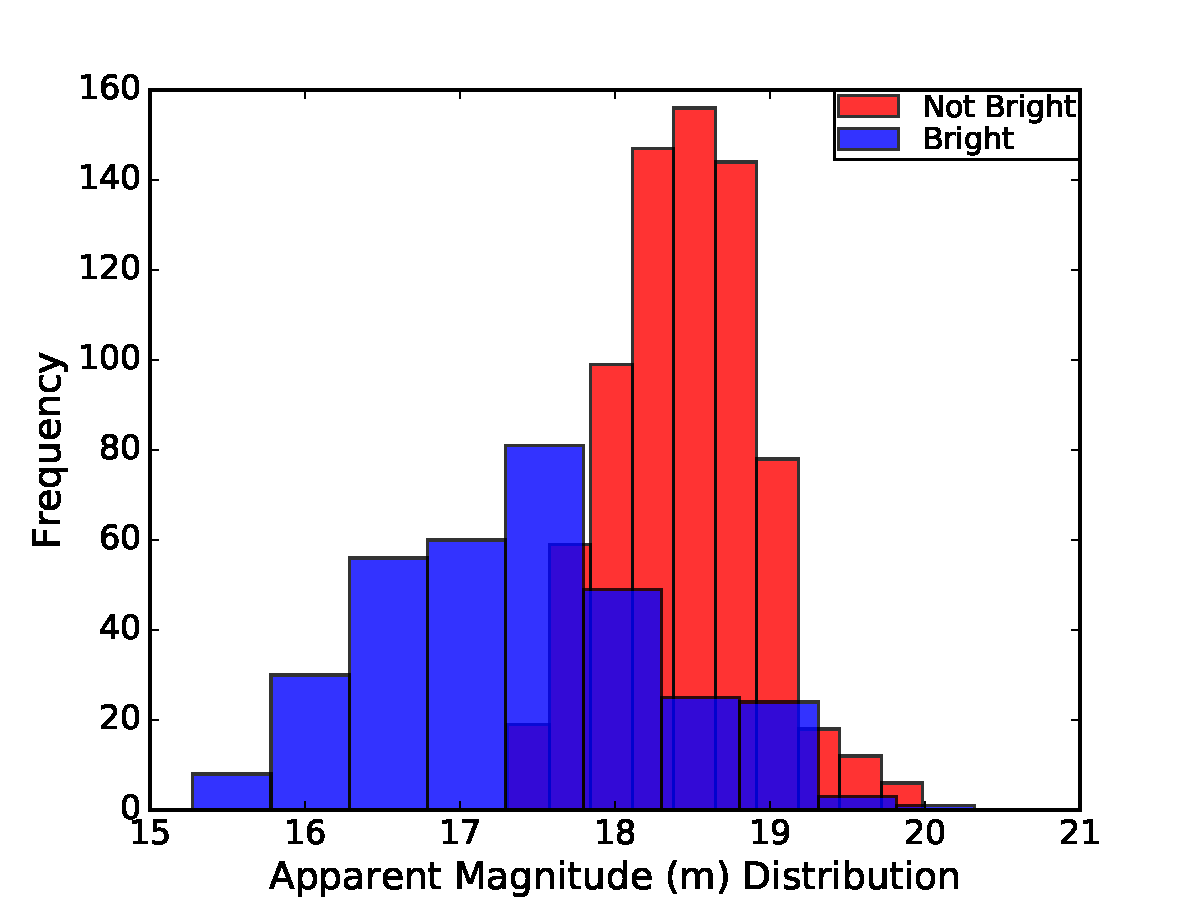
\includegraphics[width=0.5\textwidth]{3meanuplimmagdist.pdf}}
\hfill
\subfloat[Redshift (Z) Distribution\label{subfig:sfig12}]{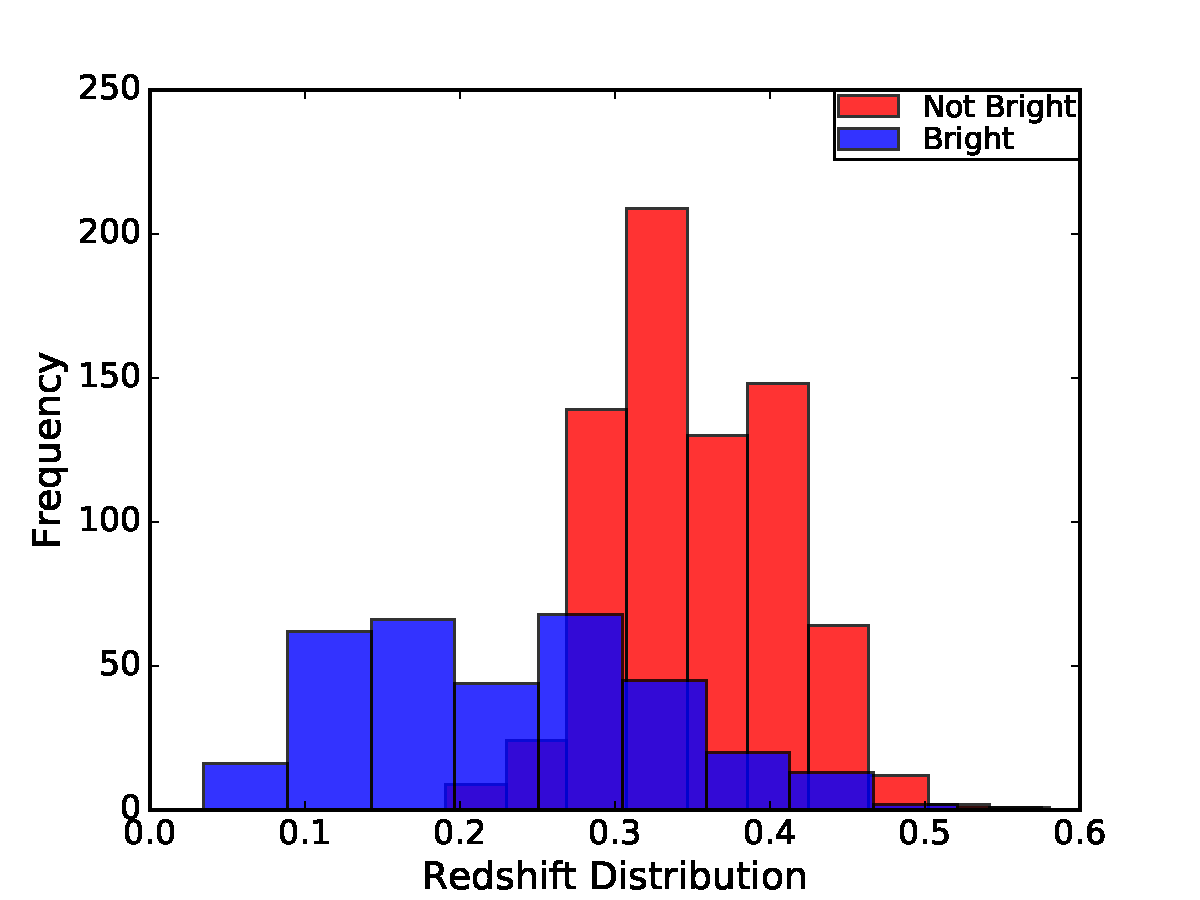
\includegraphics[width=0.5\textwidth]{3meanuplimzdist.pdf}}
 \caption{With redshift cut: Apparent magnitude and redshift distributions for LRG's flagged as Bright Center Objects (blue bars), and those not flagged as Bright Center Objects (red bars). }
\label{fig:mesha1}
\end{figure}

Since we first want to confirm that these galaxies are all from the same population, in Figure \ref{fig:mesha1}, we construct the distributions of the redshifts and apparent apparent magnitudes for flagged (blue bars) and not flagged (red bars) galaxies.

Varying parts of the stacked profile use distinct galaxies at different redshifts. As seen in Figure\ref{fig:mesha1}, the apparent magnitudes and redshifts for the flagged galaxies aren't normally distributed like the non-flagged galaxies. While the blue bars trail off at m=17, we also notice that they trail off at z=0.2. Since these galaxies were of lower redshift (as seen in Figure \ref{subfig:sfig12}), they appear to be more luminous (as seen in Figure \ref{subfig:sfig11}.) Since we are measuring intrinsic brightness, our stacked profile was falsely brighter.This is evidence that those LRGs are flagged as Bright Objects because they offset our stacked profile. Therefore, we set a lower limit of 0.2 to our redshift distribution.  

\begin{figure}[h!]
\centering
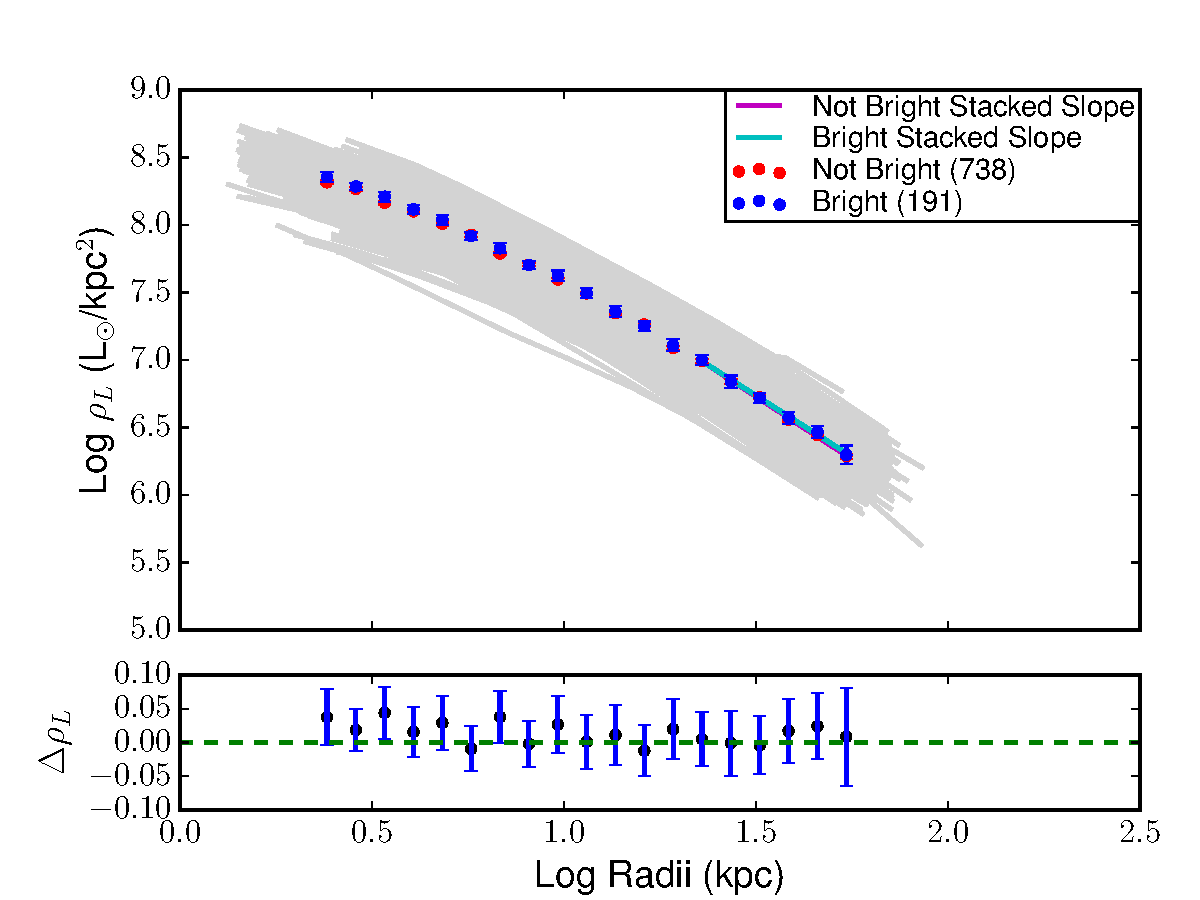
\includegraphics[width=.8\textwidth]{3+meanuplimTF.pdf}
\caption{The luminosity profiles of Bright galaxies (blue points) and not bright galaxies (red points)}
\label{fig:mesh1}
\end{figure}


Figure \ref{fig:mesh1} shows stacked luminosity profile for each flagged (blue points) and non-flagged populations (red points). In the background, I plot the luminosity profiles of the individual galaxies (gray curves).  In order to homogenize our results, so they are all fit to the same physical boundary, we set an inner boundary of $3R_{1/2}$ and an outer boundary of exactly $6R_{1/2}$ to both individual luminosity profiles and stacked profiles. 

Typically, the half light radius ($R_{1/2}$) marks the inner boundary of the stellar halo. However, since HSC can probe to very low surface brightness, we wanted to use this tool to our advantage and only look at the outermost regions of the stellar halo. Also, in Pillepich et al, the outer boundary was marked by the virial radius ($R_{vir}$). Since we found that $R_{vir}$ for our galaxies extended beyond our largest measured aperture, we arbitrarily choose $6R_{1/2}$.  By implementing this outer limit, we can safely use photometry of these bright sources.

Interestingly,  in Figure \ref{fig:mesh1}, we see that galaxies flagged as bright objects are in agreement with those not flagged. Therefore, we can conclude that it is not necessary to disregard LRGs flagged as "Bright Objects" from our sample population. 

\section{Star Formation History via VESPA}
As galaxies merge, they accumulate more mass, and visible aspects of the stellar envelope are affected (i.e. the distribution of stars). However, the dark matter is also tidally disrupted. Since LRGs are all early-type galaxies, they have undergone mergers and accumulated most of their mass at this time.

Before we can assess the relationship between Mass Assembly and the Dark Matter envelope, we first need to see if there is a correlation between mass assembly and star formation history (SFH). Using VESPA, an algorithm that fits the spectra of all LRGs in the Sloan Digital Sky Survey's (SDSS) final data release, we match with our original catalogue to get their total spectral data, such as SFH.

\begin{figure}[h!]
\centering
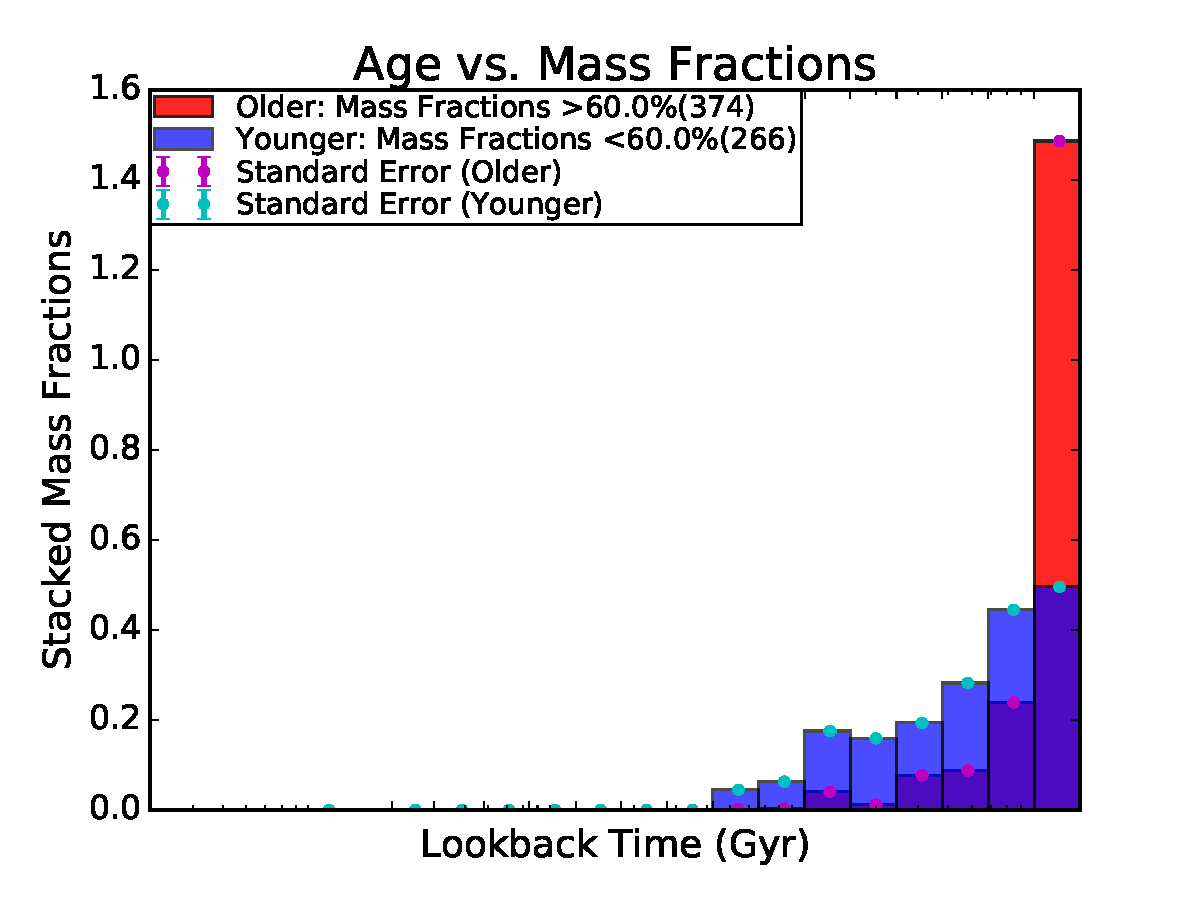
\includegraphics[width=.8\textwidth]{oy_agebin.pdf}
\caption{The mass assembly histories of older galaxies (red bars) and younger galaxies (blue bars).}
\label{fig:meshba}
\end{figure}

After matching this catalogue with the LOWZ galaxies, we next separate the LRGs into two different populations, based on whether or not 60\% of the mass of the galaxy is formed in the oldest age bin (between 9.06 and 14 billion years ago), as seen in Figure \ref{fig:meshba}. It is important to note that these are all early type galaxies, but we can still distinguish them by SFH based on when they accumulated the most mass. .


\begin{figure}[h!]
\centering
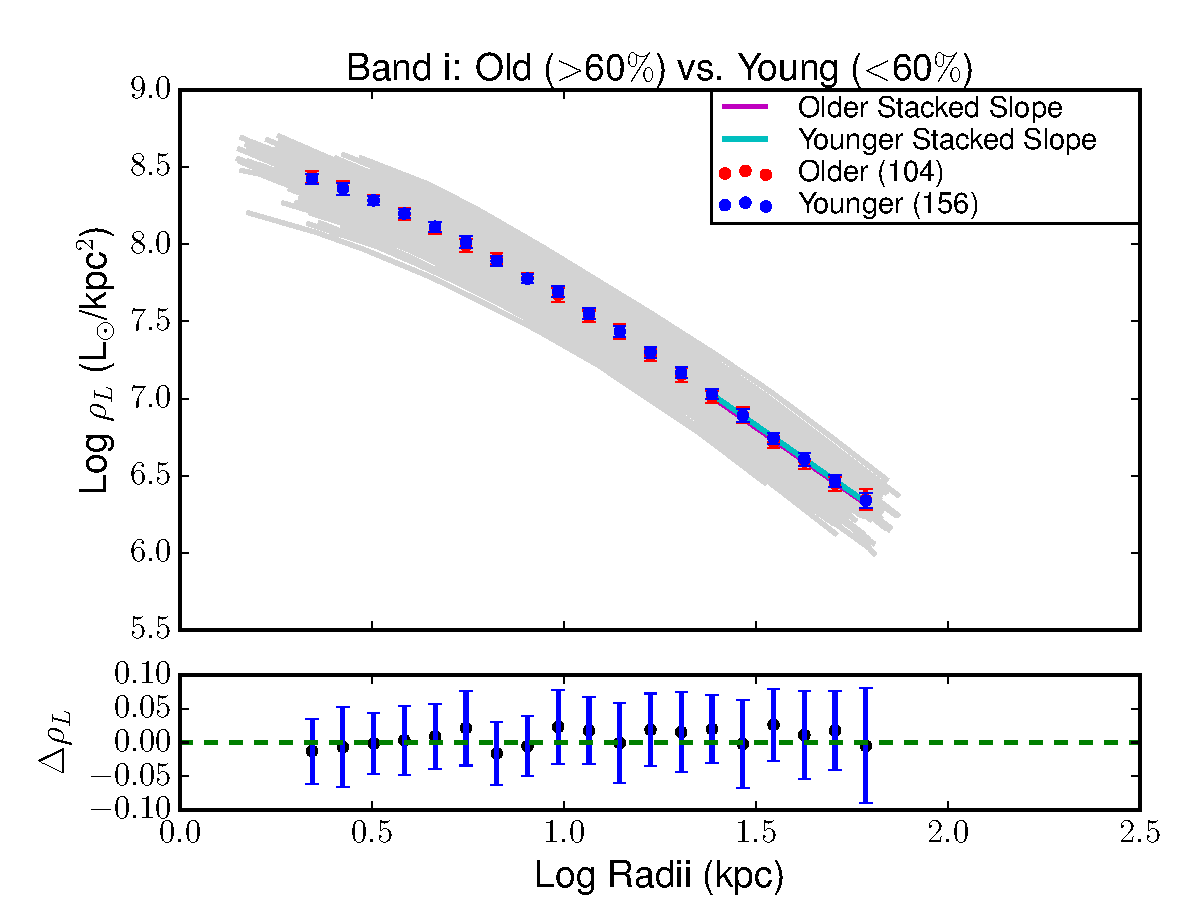
\includegraphics[width=.8\textwidth]{3+oymeanuplimlumage.pdf}
\caption{The luminosity profiles of older galaxies (red points) and younger galaxies (blue points).}
\label{fig:mesh2}
\end{figure}

As seen in Figure \ref{fig:mesh2}, when plotting the luminosity profiles for older and younger LRGs,  the stacked slopes appear to be roughly the same.

\begin{table}[!htb]
\centering
\begin{tabular}{ccc} \toprule
& \Large{\textbf{\textbf{$\alpha_{stars}$}}}\\ \midrule
\textbf{Old Galaxies} & \textbf{-1.73  $\pm$  0.142}  \\
\textbf{Young Galaxies} & \textbf{-1.746 $\pm$  0.12}\\
Old and Not Flagged & -1.765 $\pm$  0.1 \\
Old and Flagged & -1.586  $\pm$  0.221 \\
Young and Not Flagged & -1.786 $\pm$  0.094 \\
Young and Flagged & -1.645  $\pm$  0.299 \\ \bottomrule
\end{tabular}
\caption{These stacked slopes ($\alpha_{stars}$) were calculated from specific population's individual galaxy slope distribution}
\label{table:3}
\end{table}

It is important to note that about half of the LRGs in the older and younger samples are flagged as Bright Objects. In Table \ref{table:3}, we show the Bright and Not Bright stacked slopes for every subsample. Since the stacked slopes of every subgroup coincides with the older and younger galaxies' slopes within one $\sigma$, we can confirm that the flag has little effect on the overall luminosity profile.

\begin{figure}[h!]
\centering
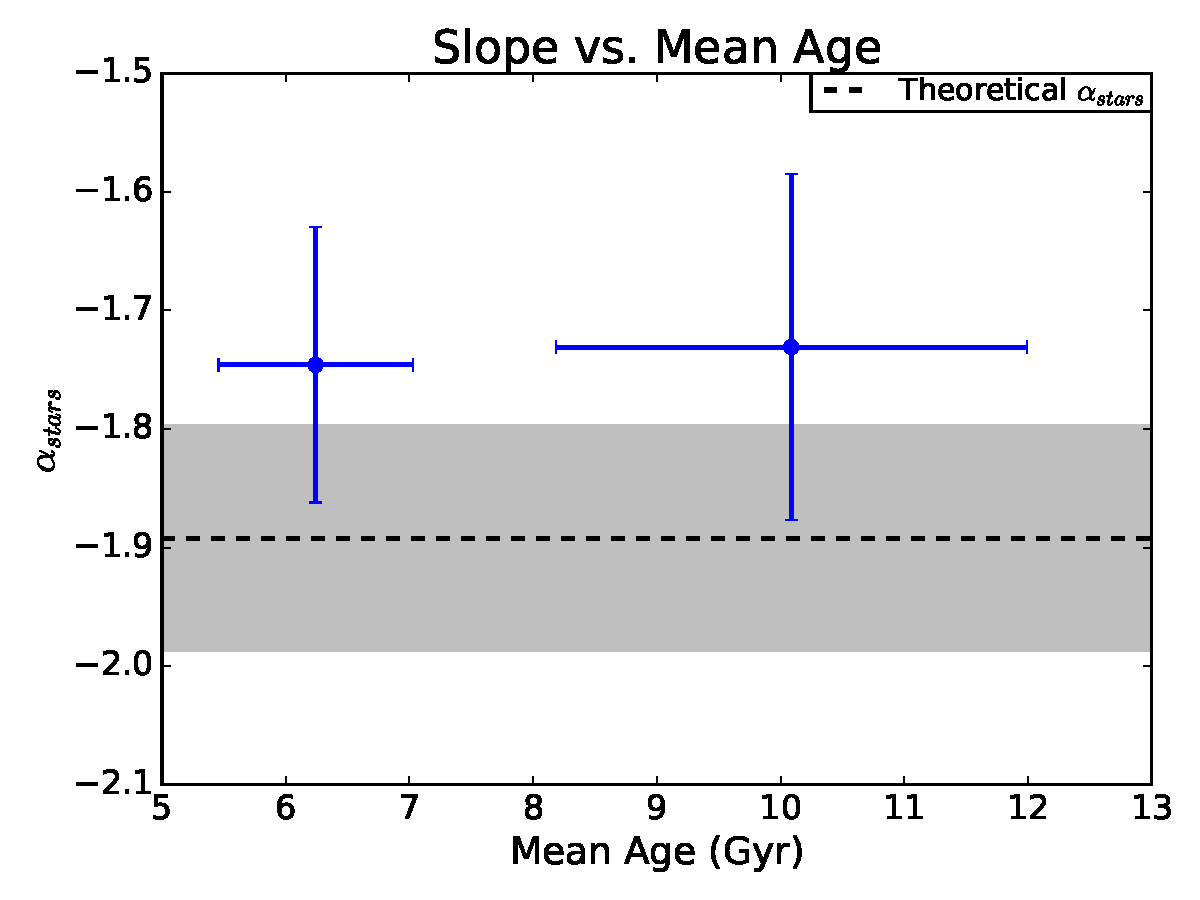
\includegraphics[width=.8\textwidth]{slopevmed.pdf}
\caption{The stacked slope ($\alpha_{stars}$) and mean age (blue points). The black dotted line represents the theoretical  $\alpha_{stars}$}
\label{fig:svm}
\end{figure}

As a final representation, Figure \ref{fig:svm} shows the relationship between mean age and slope. Pillepich plotted the theoretical luminosity density to comoving distance for elliptical galaxies. As a frame of reference, we found the theoretical  $\alpha_{stars}$ for the same stellar envelope range we used in our stacked slopes.

We found that  $\alpha_{stars}$ is not dependent upon its formation time. It is also within $1\sigma$ of what we expect to get, according to Pillepich. 


\section{Conclusion}

In conclusion, it is not necessary to remove bright objects (as long as we fit $\alpha_{stars}$ to the same physical range). We also found no correlation between accretion history and Star formation epoch, as determined by $\alpha_{stars}$. 

The next step is to use Weak Gravitational Lensing to get the total halo mass, and ultimately find the relationship between $\alpha_{stars}$ and the Dark Matter Halo.

This experiment can be varied. For example, we are only using one of HSC's six Wide Fields. We can expand to one of the other fields to compare our results. Furthermore, we can use a different galaxy population. LRGs might contain too narrow of a Star Formation History range. We might want to try younger, more active, bright galaxies, such as CMASS.


\end{document}